%\setchapterimage{fig_00}
\chapter*{Colle \arabic{cptColle} \\
Robot MIR : Machine d'inspection des réacteurs rapides -- \ifprof Corrigé \else Sujet \fi}

\addcontentsline{toc}{section}{Colle \arabic{cptTD} : Robot MIR : Machine d'inspection des réacteurs rapides -- \ifprof Corrigé \else Sujet \fi}

\iflivret \stepcounter{cptColle} \else
\ifprof  \stepcounter{cptColle} \else \fi
\fi
\setcounter{question}{0}

\marginnote{E3A MP -- 2012.}
\begin{marginfigure}
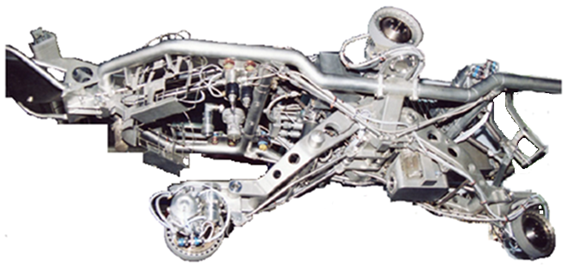
\includegraphics[width=\linewidth]{mir_01}
\end{marginfigure}


\subsection*{Mise en situation}

%\begin{minipage}[c]{.25\linewidth}
%\begin{center}
%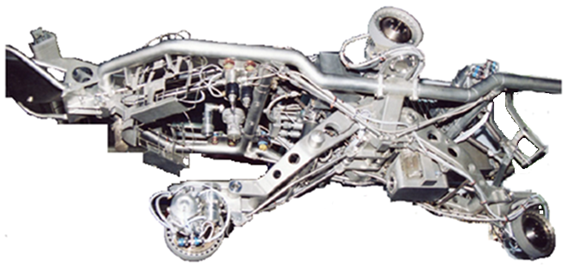
\includegraphics[width=.9\linewidth]{mir_01}
%\end{center}
%\end{minipage} \hfill
%\begin{minipage}[c]{.7\linewidth}
Le robot MIR développé pour la vérification des cuves de Superphenix doit être adapté pour le contrôle d’une nouvelle génération de réacteurs à neutrons rapides.

L’objectif du robot MIR est de :
\begin{itemize}
\item assurer le contrôle surfacique télévisuel des soudures des deux cuves et des zones adjacentes ;
\item assurer le contrôle volumique par ultrasons des soudures de la cuve principale et des zones adjacentes. Une possibilité était offerte d’effectuer ce contrôle sur la cuve de sécurité ;
\item mesurer en permanence la distance entre les deux cuves.
\end{itemize}

%\end{minipage} 

%Le robot MIR est un véhicule motorisé composé d’un châssis tubulaire, de quatre bras articulés et des composants nécessaires à la mise en œuvre des contrôles et mesure. La structure est en acier inoxydable. La masse est d’environ 180 kg.
%
%À l’extrémité de chaque bras, se trouve une roue motorisée en rotation et en direction. Il y a donc au total 4 roues qui servent d’appui contre les parois de cuve (principale et de sécurité).
%
%Sur la partie inférieure, sont situés le mini bac d’inspection et son système de plaquage. Ce sous-ensemble constitue le dispositif d’inspection proprement dit. Le rôle dévolu au reste du robot étant de positionner le mini bac d’inspection au droit de la soudure à contrôler.
%La chaîne d’énergie associée au déplacement
%Chaque roue utilise un module de déplacement. Il y a quatre modules de déplacement sur le robot MIR, pilotant le déplacement.
%Chaque module est composé d’un corps, d’une roue, du motoréducteur de traction, du motoréducteur d’orientation et du potentiomètre d’orientation.
%La roue est la pièce tournante en contact avec les parois de la cuve. La surface extérieure torique est revêtue d’une couche mince de carbure de tungstène déposé par projection plasma. Ce revêtement est très tenace et présente l’avantage d’avoir un coefficient de frottement sur l’acier inoxydable élevé ($f \geq 0,5$).
%
%
%\subsection*{Étude de la fonction : Synchroniser les vitesses des roues}
%
%On se place au niveau de l’arbre moteur avant réduction, couples et vitesses ramenées sur l’arbre moteur.
%
%\begin{obj}
%Synchroniser les vitesses des roues.
%\end{obj}
%La synchronisation automatique de la vitesse des quatre roues est basée sur la parfaite réversibilité de la transmission des efforts de la roue vers le réducteur puis le moteur. 
%
%%Ceci se concrétise par le fait que, pour une consigne de vitesse donnée, le contrôle-commande envoie la même tension aux bornes des quatre moteurs. La synchronisation s'effectue alors par les variations imposées au courant moteur. 
%%
%%Par exemple si un motoréducteur a tendance à induire une vitesse supérieure à celle imposée par le déplacement de l'engin, cette tendance se traduit par un couple moteur plus grand, donc par une augmentation de l'intensité qui induit elle-même une diminution de la vitesse jusqu'à la valeur permise.
%%
%%Ce principe qui permet un contrôle-commande relativement simple exige en contrepartie une réversibilité parfaite de fonctionnement du réducteur, toute dégradation de cette réversibilité entraînant rapidement un fonctionnement chaotique de l'engin.
%
%Dans une première approche, on ne s’intéresse qu’aux roues inférieures \textbf{SA} et \textbf{SB}.
%
%Les roues \textbf{SA} et \textbf{SB} sont munies des mêmes motoréducteurs avec les mêmes moteurs à courant continu.
%Elles sont commandées en tension sur l’induit. Les circuits d’induit ont la même résistance $R$ et une inductance négligeable.
%
%On s’intéresse d’abord au moteur de la roue \textbf{SA} seule.
%
%On notera :
%\begin{itemize}
%\item $\omega_{mA}(t)$ : vitesse angulaire de rotation à la sortie du moteur, avant réduction (en $\text{rad}\text{s}^{-1}$);
%\item $c_{mA}(t)$ : couple exercé par le moteur de la roue \textbf{SA} sur l’arbre moteur en N.m;
%\item $c_{mB}(t)$ : couple exercé par le moteur de la roue \textbf{SB} sur l’arbre moteur en N.m;
%\item $J$ : moment d’inertie équivalent en $\text{kg}{m}^2$.
%\end{itemize}
%Rappelons les équations régissant le moteur : 
%\begin{itemize}
%\item équations électriques (en négligeant l’effet de l’inductance) : $u(t)=Ri_A(t)+e_A(t)$;
%\item équation mécanique issue de l’étude précédente, ramenée à l’arbre moteur de la roue \textbf{SA} : $c_{mA}(t)+c_{mB}(t)=J\dfrac{d\omega_{ma}(t)}{dt}$;
%\item équations électromécaniques : $e_a(t)=K_A\omega_{mA}(t)$ et $c_{mA}(t)=K_Ai_A(t)$.
% \end{itemize}
% 
%L’entrée du système est la tension de commande appliquée aux bornes du moteur, la sortie est la vitesse de rotation de la roue \textbf{SA}, on peut modéliser le système à l’aide du schéma bloc suivant :
%\begin{center}
%	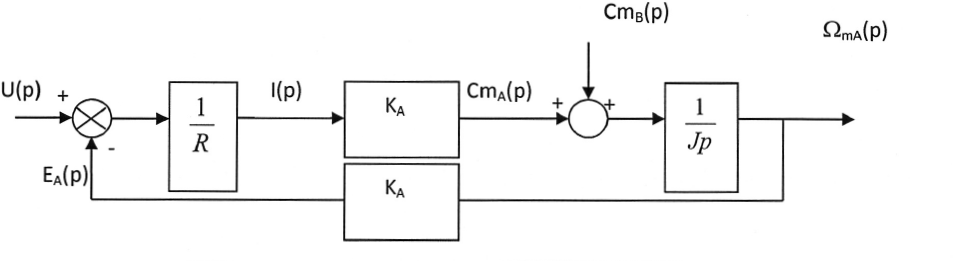
\includegraphics[width=\linewidth]{fig_10}
%\end{center}
%
%
%
%\subparagraph{}
%\textit{Exprimer la fonction de transfert $\dfrac{\Omega_{mA}(p)}{U(p)}$ lorsque $C_{mB}(p)=0$ et la mettre sous forme canonique.}
%\ifprof
%\begin{corrige}
%\end{corrige}
%\else
%\fi
%
%
%\subparagraph{}
%\textit{Exprimer quelle serait la valeur finale de la vitesse de rotation du moteur raccordé à la roue \textbf{SA}, notée $\omega_{mAf0}$ si on considère que $C_{mb}(p)=0$, et ceci pour une entrée modélisée par un échelon de tension d’amplitude $u_0$.}
%\ifprof
%\begin{corrige}
%\end{corrige}
%\else
%\fi
%
%
%\subparagraph{}
%\textit{Exprimer la fonction de transfert $\dfrac{\Omega_{ma}(p)}{C_{mb}(p)}$ lorsque $U(p)=0$ et la mettre sous forme canonique.}
%\ifprof
%\begin{corrige}
%\end{corrige}
%\else
%\fi
%
%Si les deux roues fonctionnent à la même vitesse, on a la structure du schéma bloc de la figure 10 pour chacune des deux roues.
%
%Mais si les moteurs ont une légère différence, par exemple la constante électromécanique $K_A$ et $K_B$, les 2 roues prendraient des vitesses différentes. Mais contraintes par le châssis et l’adhérence aux parois à tourner à la même vitesse (en ligne droite), elles exercent l’une sur l’autre un effort qu’on peut ramener à l’arbre moteur sous forme d’un couple supplémentaire $C_{mB}$ sur la roue \textbf{SA}, et $C_{mA}$ sur la roue \textbf{SB}. On a alors le schéma suivant :
%\begin{center}
%	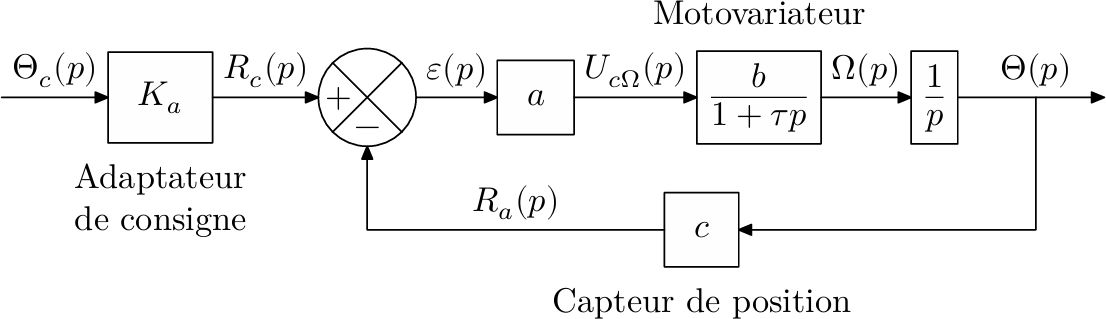
\includegraphics[width=\linewidth]{fig_11}
%\end{center}
%
%\subparagraph{}
%\textit{Exprimer la fonction de transfert globale sous forme canonique : $\dfrac{\Omega_m(p)}{U(p)}$.}
%\ifprof
%\begin{corrige}
%\end{corrige}
%\else
%\fi
%
%
%\subparagraph{}
%\textit{Si l’entrée est un échelon de tension d’amplitude $u_0$, calculer la valeur finale de la vitesse de rotation de chacun des moteurs, notée $\omega_\text{finale}$. Conclure quant à la possibilité d’avoir roulement sans glissement entre chacune des roues et les cuves.}
%\ifprof
%\begin{corrige}
%\end{corrige}
%\else
%\fi

\subsection*{Étude de la fonction Ft12 : Déplacer le transducteur à vitesse constante}
\ifcolle
\else
Le robot MIR étant à l’arrêt entre les deux cuves, le mini bac est plaqué contre la paroi de la cuve à contrôler. Pour l’inspection des soudures, le transducteur 13 (capteur de l’état des soudures) doit se déplacer à l’intérieur du mini bac d’inspection à vitesse constante. Le mini bac est rempli d’un fluide visqueux. L’inspection peut avoir lieu pour n’importe quelle position du robot MIR, donc l’angle $\alpha$ qui caractérise la direction du déplacement du transducteur par rapport à l’horizontale, est susceptible de prendre toute valeur comprise entre $-\pi/2$ (robot tête en bas) et $\pi/2$ (robot tête en haut). Afin de garantir la qualité des résultats de mesure, le transducteur doit donc se déplacer à une vitesse $V_0$ constante par rapport à la paroi, et ceci pour toute valeur de l’angle $\alpha$.
\fi

\begin{obj}
Qualifier la précision statique du système et définir les améliorations à apporter.
\end{obj}

\begin{marginfigure}
	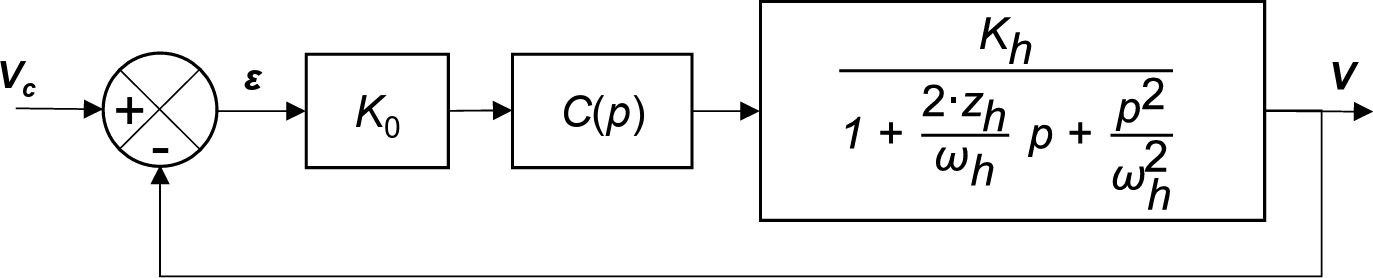
\includegraphics[width=\linewidth]{fig_12}
\end{marginfigure}

L’objectif de cette partie est de dimensionner le correcteur nécessaire au respect d’un écart statique nul, et ceci malgré le caractère variable de l’angle $\alpha$.

Le transducteur est en liaison glissière de direction $\vect{x_r}$, avec le corps \textbf{1} du robot MIR. La chaîne d’énergie est composée entre autre, d’un actionneur rotatif qui exerce un couple $c(t)$ sur le pignon \textbf{11}, qui est en liaison pivot, supposée parfaite, avec le robot MIR.
Un système poulies (\textbf{11} et \textbf{12}) et courroie crantée \textbf{14} impose le mouvement de translation au transducteur \textbf{13}.
 
 Le comportement dynamique du système est régit par l'équation suivante  :
 $$
 M_{eq}\dfrac{\text{d}v_r(t)}{\text{d}t}=\delta c(t) + \beta v_r(t) + \gamma g u(t)
 $$
avec $u(t)$ échelon unitaire.

On cherche à garantir une vitesse de translation du transducteur \textbf{13} égale à la valeur de consigne indépendamment de l’angle $\alpha$.

Pour cela, on réalise le système bouclé suivant :

\begin{center}
	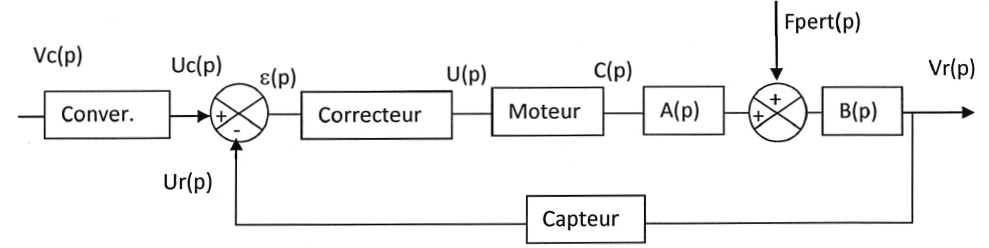
\includegraphics[width=\linewidth]{fig_13}
\end{center}

%Notations : $V_r(p)$ est la transformée de Laplace de $v_r(t)$ vitesse de translation du transducteur \textbf{13}.
%$F_{\text{pert}}(p)$ est la transformée de Laplace de $f_{\text{pert}}(t)$, avec :
%$f_{\text{pert}}(t) = -m_t  \sin \alpha u(t)$ avec $u(t)$ échelon unitaire.


\question{En supposant des conditions initiales nulles, exprimer les fonctions de transfert $A(p)$ et $B(p)$ en fonction entre autres de $\delta$, $\beta$ et $M_{eq}$.
}
\ifprof
\begin{corrige}
\end{corrige}
\else
\fi


Le capteur est modélisé par un gain pur de valeur $K_{\text{capt}}$.

\question{En supposant une perturbation nulle, quelle doit être la valeur du gain $K_{\text{conv}}$ du convertisseur modélisé par un gain pur, afin que l’écart $\varepsilon(t)$ soit nul quand la valeur de la vitesse réelle $v_r(t)$ est égale à la valeur de la consigne $v_c(t)$. }
\ifprof
\begin{corrige}
\end{corrige}
\else
\fi
On adopte pour la suite la modélisation suivante :

\begin{center}
	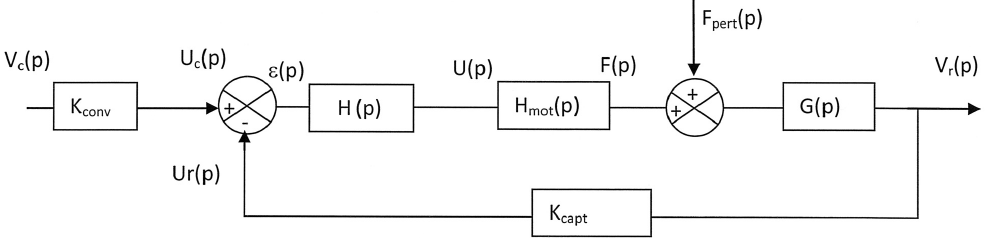
\includegraphics[width=\linewidth]{fig_14}
\end{center}

Avec $H_{\text{mot}}(p)=\dfrac{K_m}{1+\tau_m p}$, $G(p)=\dfrac{K}{1+\tau p}$ et $H(p)=K_{\text{cor}}$ fonction de transfert du correcteur.


\question{Exprimer les deux fonctions de transfert : $H_1(p)=\left(\dfrac{V_r(p)}{V_c(p)} \right)_{F_{\text{pert}}(p)=0}$ et $H_2(p)=\left(\dfrac{V_r(p)}{F_{\text{pert}}(p)} \right)_{V_c(p)=0}$ en fonction des gains $K_\text{\text{conv}}$, $K_{\text{cor}}$, et $K_{\text{capt}}$ ainsi que des fonctions de transfert $H_{\text{mot}}(p)$ et $G(p)$.}
\ifprof
\begin{corrige}
\end{corrige}
\else
\fi

\question{En supposant que $K_{\text{cor}}= 1$ et en indiquant les valeurs remarquables, tracer les diagrammes asymptotiques dans le plan de Bode de la fonction de transfert en boucle ouverte $\dfrac{U_r (p)}{\varepsilon(p)}$ en utilisant les valeurs numériques suivantes :}
$K_m = \SI{0.1}{N.V^{-1}}$, $\tau_m= \SI{0,01}{s}$, $K_{\text{capt}} = \SI{50}{V.s.m^{-1}}$, 
$K = \SI{200}{m.s^{-1}.N^{-1}}$, $\quad \tau = \SI{1}{s}$.

\ifprof
\begin{corrige}
\end{corrige}
\else
\fi


\question{Déterminer le gain en décibel de la fonction de transfert en boucle ouverte (courbe réelle) pour la pulsation de \SI{100}{rad.s^{-1}}.}
\ifprof
\begin{corrige}
\end{corrige}
\else
\fi


On formule l’hypothèse simplificatrice suivante : la phase de la fonction de transfert en boucle ouverte pour une pulsation de 100 rad/s est de $-135\degres$.


\question{On souhaite une marge de gain \SI{12}{dB} et un marge de phase de 45\degres, en utilisant le résultat de la question précédente, déterminer la valeur numérique correspondante de $K_{\text{cor}}$.
Commenter la valeur de la marge de gain obtenue ?}
\ifprof
\begin{corrige}
\end{corrige}
\else
\fi


\question{On impose une vitesse constante en entrée de valeur $v_0$ ($v_c(t)=v_0.u(t)$) avec $u(t)$ fonction échelon unitaire de Heaviside. Exprimer l’écart statique en régime permanent en tenant compte de la perturbation (en fonction de l’angle $\alpha$, de la valeur de $K_{\text{cor}}$ et des données).}
\ifprof
\begin{corrige}
\end{corrige}
\else
\fi


On souhaite obtenir une vitesse de translation indépendante de l’inclinaison. Pour toute la suite du sujet, on installe un correcteur intégral du type $\dfrac{K_c}{p}$, placé au début de la chaîne d’action.

\question{On impose de nouveau une vitesse constante en entrée de valeur $v_0$ ($v_c(t)=v_0.u(t)$); exprimer l’expression du nouvel écart statique en régime permanent (en fonction de l’angle $\alpha$ et des données). Pouvait-on prévoir ce résultat ?}
\ifprof
\begin{corrige}
\end{corrige}
\else
\fi


\ifprof
\begin{center}
	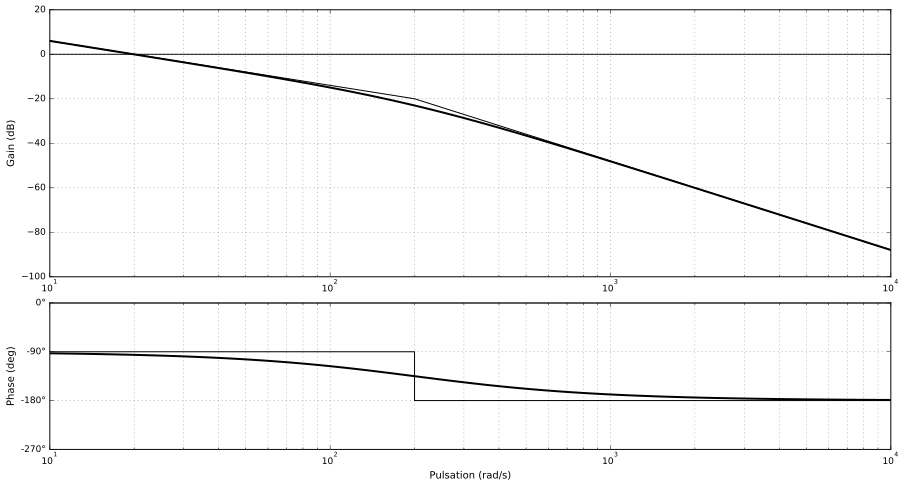
\includegraphics[width=.8\linewidth]{cor_01}
\end{center}

\begin{center}
	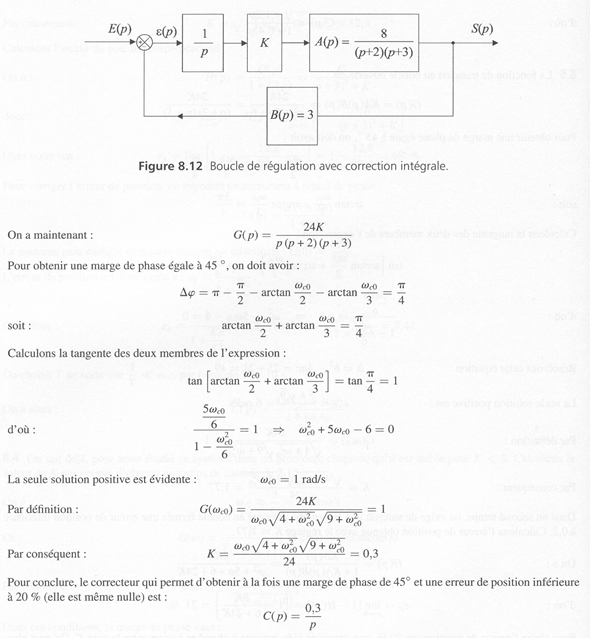
\includegraphics[width=.8\linewidth]{cor_02}
\end{center}

\begin{center}
	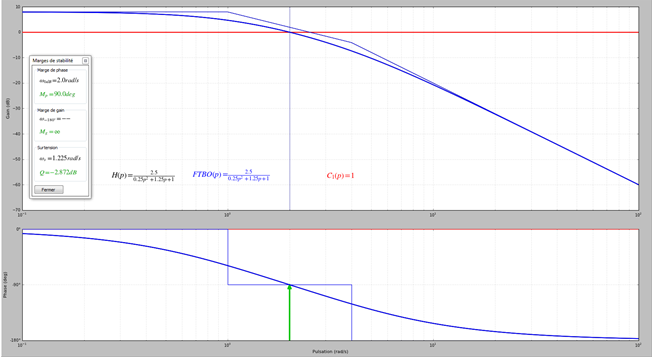
\includegraphics[width=.8\linewidth]{cor_03}
\end{center}

\begin{center}
	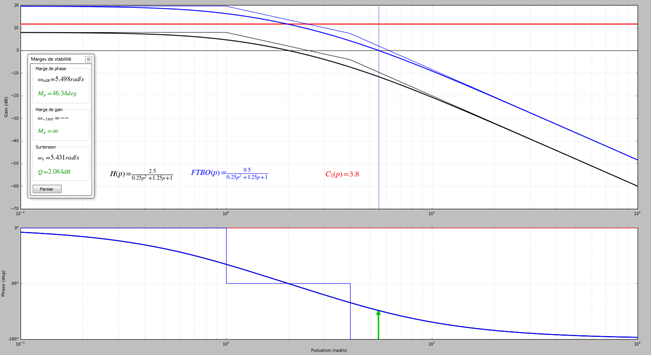
\includegraphics[width=.8\linewidth]{cor_04}
\end{center}

\begin{center}
	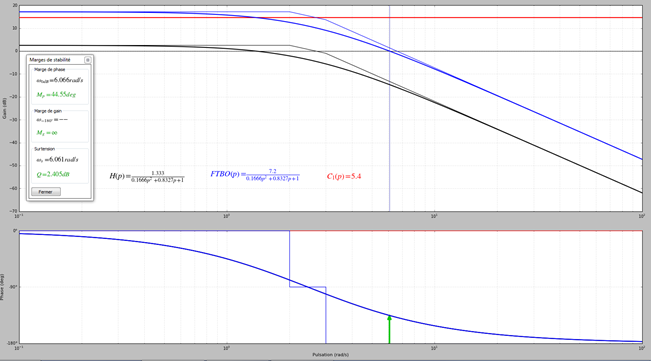
\includegraphics[width=.8\linewidth]{cor_05}
\end{center}

\begin{center}
	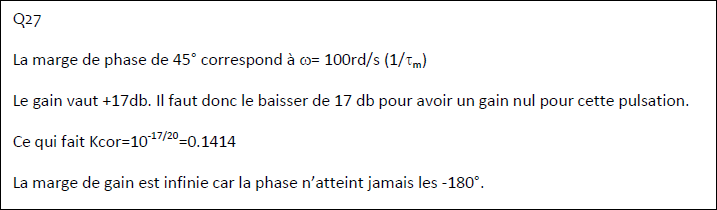
\includegraphics[width=.8\linewidth]{cor_06}
\end{center}

\begin{center}
	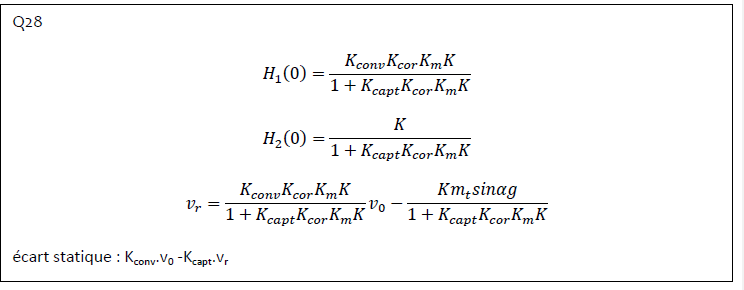
\includegraphics[width=.8\linewidth]{cor_07}
\end{center}

\begin{center}
	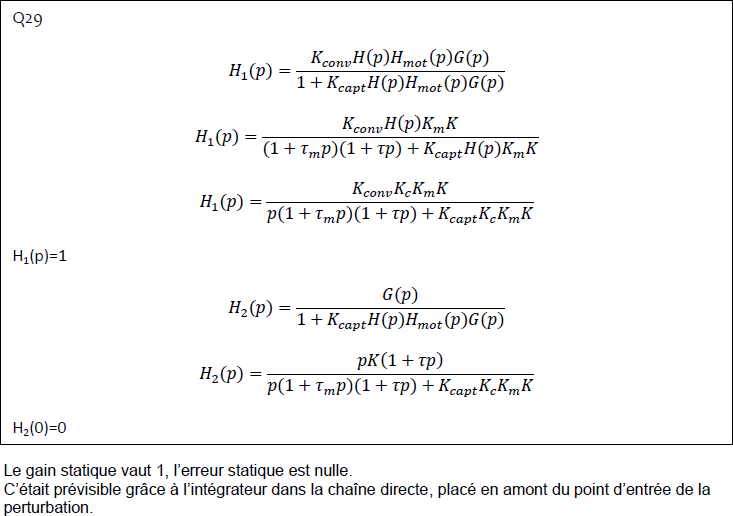
\includegraphics[width=.8\linewidth]{cor_08}
\end{center}
\else
\fi